\documentclass[a4paper, 10pt, twocolumn]{article}
% Sowohl LaTeX als auch pdfLaTeX können benutzt werden, um das Manuskript zu erstellen.

% Bitte öffnen sie diese Datei mit utf8 Zeichenkodierung!!!
\usepackage[utf8]{inputenc}         % Schriftkodierung dieser Datei
\usepackage[english]{babel}          % für deutsche Dokumente

\usepackage{graphicx}               % optional für Grafiken
\usepackage{tabularx}               % optional für Tabellen
\usepackage{multirow}               % optional für Tabellen
\usepackage{url}                % optional für Internet Links

\usepackage[small,bf]{caption2}     % bitte für Bildunterschriften verwenden
\usepackage{parskip}
\usepackage{titlesec}
\usepackage{amsmath}                % optional für Formeln

\titleformat{\section}{\normalfont\large\bfseries}{\thesection}{}{}
\titleformat{\subsection}{\normalfont\large\bfseries}{\thesection}{}{}
\titleformat{\paragraph}{\normalfont\bfseries}{\theparagraph}{}{}
\titlespacing{\section}{0pt}{6pt}{-1pt}
\titlespacing{\subsection}{0pt}{3pt}{-1pt}
\titlespacing{\paragraph}{0pt}{3pt}{-1pt}

\newcolumntype{Y}{>{\centering\arraybackslash}X}    %für Tabellen mit tabularx

% Definition der Seitenränder
\addtolength{\textwidth}{2.1cm}
\addtolength{\topmargin}{-2.4cm}
\addtolength{\oddsidemargin}{-1.1 cm}
\addtolength{\textheight}{4.5cm}
\setlength{\columnsep}{0.7cm}

\pagestyle{empty}                   % weder Kopf- noch Fußzeile auf 1. Seite

\begin{document}

\date{}                                         % kein Datum auf 1. Seite

\title{\vspace{-8mm}\textbf{\large
Assessment and Evaluation of an Unsupervised Machine Learning Model for Automotive and Industrial NVH Applications }}

% Hier die Namen und Daten der beteiligten Autoren eintragen
\author{
Abdul Haq Azeem Paracha$^1$, Johannes Blickensdorff$^2$, Dr. David Scott Johnson$^3$ \\
$^1$ \emph{\small Technische Universität Ilmenau, 98693 Ilmenau,
Germany, Email: abdulhaq.ah@gmail.com
}\\
$^2$ \emph{\small Schaeffler Technologies AG \& Co. KG, Germany,
Email: blickjha@schaeffler.com 
}\\ 

$^3$ \emph{\small Fraunhofer IDMT, 98693 Ilmenau, Germany,
Email: david.scott.johnson@idmt.fraunhofer.de}

}
\maketitle
\thispagestyle{empty}           % weder Kopf- noch Fußzeile auf Folgeseiten
% Beginn des eigentlichen Manuskripts


\section*{Abstract}
\label{sec:Abstract}
Current NVH analysis techniques involve an interdisciplinary knowledge of structural dynamics, signal processing, technical- and psychoacoustics but most notably they require an experienced professional to analyse and assess the ever-expanding amount of acquired industrial NVH data.
Recent advances in machine learning have shown the possibilities of inference on feature representations of input data without human intervention, which has significantly helped experts to focus on actual solutions and reduce manual efforts for preprocessing and classification \cite{b1}.

\section*{Introduction}
\label{sec:Introduction}

Machine learning (ML) algorithms provide key methods to improve the ability of machines to learn from data. The main idea behind machine learning is inductive inference, through which specific statistical phenomena are generalized \cite{b2}. Rapid changes in the global industry, like the emergence of the electric vehicles and high resolution data, have posed serious challenges for NVH engineers. The here so called "classical approaches" require an in depth assessment of time and frequency data by an human expert with well known signal processing techniques to confirm and validate NVH properties of specimen with respect to hardware design, root causes and simulation results. Nevertheless we challenged we challenged an unsupervised deep neural network (DNN) model based on autoencoders (AE) to detect anomalies in industrial NVH data and compared findings with classically annotated data by an NVH expert \cite{b3}. 
Figure \ref{fig:types_of_ml} shows a stem overview of ML methods where an unsupervised AE was used for this research.  

\begin{figure}[hbt]
    \begin{center}
        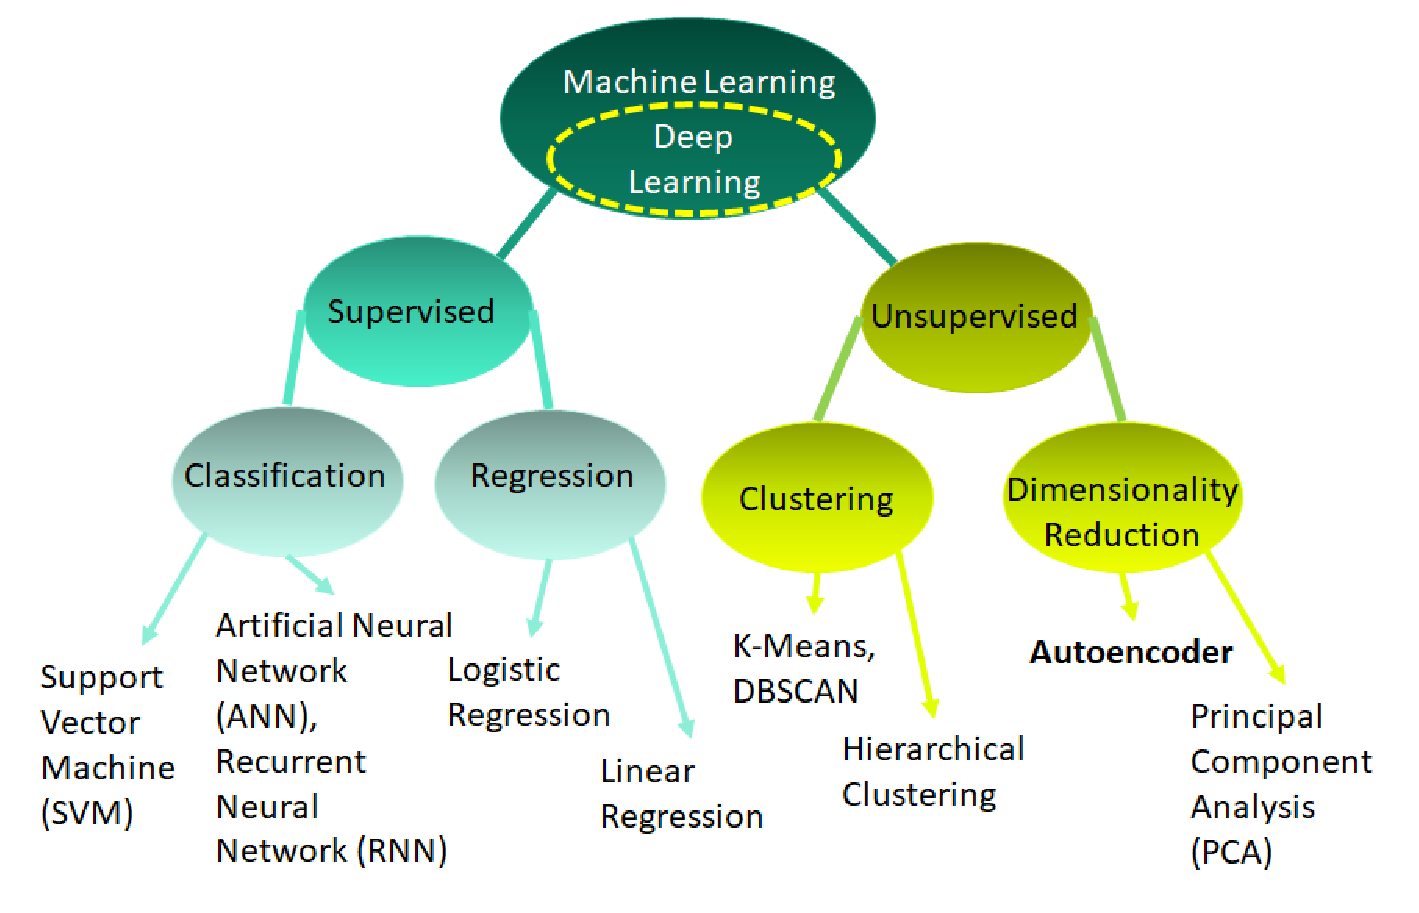
\includegraphics[width=9cm]{ml_types.eps}
    \end{center}
    \caption{Types of machine learning algorithms}
    \label{fig:types_of_ml}
\end{figure}

\section*{Related Work}
\label{sec:Related Work}
The current industrial approaches reduce the complexity of acoustical parameters to a set of basic principles for a definition of metrics which represent target characteristics for electric drive units (EDU) \cite{b4}. In comparison to a "manual" feature extraction (FE) through e.g. short time fourier transform (STFT) and order based analyses, DNN provide an alternative approach of extraction, learning and analysis of features and whole system representations. They have shown significant success in image and speech recognition applications but the ML algorithm performance is greatly dependent on the choice of data features \cite{b1}. Therefore this research was focused on a comparison of STFT and order features to an AE model having the same architecture and hyperparameter configurations. We compare the effectiveness of DNN methods to benchmark classical NVH analyses where data was annotated by an NVH expert.  

\section*{Dataset}
\label{sec:Dataset}
Industrial NVH datasets include airborne and structure borne noise, multichannel data in most cases with different sampling rates from mid to high range (e.g. 100 kHz for short time impulse assessment). Therefore the used datasets have triaxial multichannel time series data from different measurement points (MP) that also include reference data channels like temperature, torque and rotational speed. The first NVH R\&D dataset has a small number of devices under test (DUT) and many channels while the second end of (production) line (EoL) dataset has a larger number of DUT’s but less channels.  Furthermore it consists of 77 gear samples in total, where 70 samples were identified as "accepted" (normal) and seven samples as "refused" through classical fault diagnosis by quality control targets. Each EoL measurement contains a total of 6 channels: Acceleration time data was acquired by one triaxial sensor that was fixed at the test bench and one additional single axis tactile sensor that was automated and touches the specimen surface. Reference channels are torque and rotational speed.  

\section*{Methodology}
\label{sec:Methodology}
For the evaluation of the AE multilayer perceptron (MLP) model on the EoL dataset, usually three steps are required: pre-processing, training and analysis. The dataset is divided into three subsets: Training,  validation and test data. A most significant step in the evaluation of AE is to train the model only on normal data. Therefore it was ensured to keep training and validation data separate from the refused specimen data. Training and validation data include all normal specimen while the test data include also refused specimen. Loss or cost function used in AE is mean squared error (MSE) which was minimized between input and output to reconstruct the data sample in latent space by adding a penalty (reduced dimension layer in the encoder) on the model. MSE are commonly used in AE applications because their efficiency and simplicity make them a good choice as a starting point \cite{b5}. The mean absolute error (MAE) was calculated between original input data and predicted output data to find the reconstruction error. As performance metric the area under curve (AUC) of precision and recall curves was used. Furthermore, based on the distribution of reconstruction errors, the overlap of normal and refused specimen data was separated by a threshold that was defined by the intersection point of precision and recall curves. Finally, the confusion matrix was used to visualize the true positives.


\section*{Toolschain}
\label{sec:Toolschain}
 The model is implemented in Tensorflow using Keras API and STFT features are extracted directly in Python piplines while order features had to be calculated in Matlab. To process the provided industrial datasets with Python the orignally supplied ASAM-ATFX transport files were converted to ASAM-MDF4 format \cite{b6}.     
 
 \section*{Experimental Setup}
\label{sec:Experimental Setup}
One data channel is used along with a rotational speed channel in the preprocessing step, order and STFT features were extracted. The procedure of anomaly detection demands test data or new data to be predicted by the model, including both: Accepted and refused specimen. Therefore 63 out of 70 normal samples were used for training and validation. Each of the seven normal and seven refused samples were used in the test subset. A relatively low number of samples indicates a deliberate effort to evaluate the performance of the model in less specimen R\&D data conditions. After feature extraction, all data were scaled through min-max normalisation to keep them in a certain range for the objective function to work properly. Architecture of the AE is primarily inspired from \cite{b7}, but modified with a number of preliminary experiments with different layer- and hyper parameter configurations. The model used for training uses rectified linear activation function (ReLU) as activation that has 10 fully connected layers. The first layer of the encoder starts with 256 neural units and progressively decreases to 16 units in the latent space. The decoder starts with 16 units and increases to 256 units in the last layer. The optimization algorithm used is Adam and learning rate is 0.0001 \cite{b8}.

\section*{Results and Discussion}
\label{sec:Results and Discussion}
There were two experiments conducted with the same model parameters, experiment A (STFT) and experiment B (orders features). Training and validation loss of the model for both experiments is 0.04, threshold of experiment A according to precision and recall vs. threshold curve is 0.169 as shown in Figure \ref{fig:threshold_expa}.

\begin{figure}[t]
    \begin{center}
        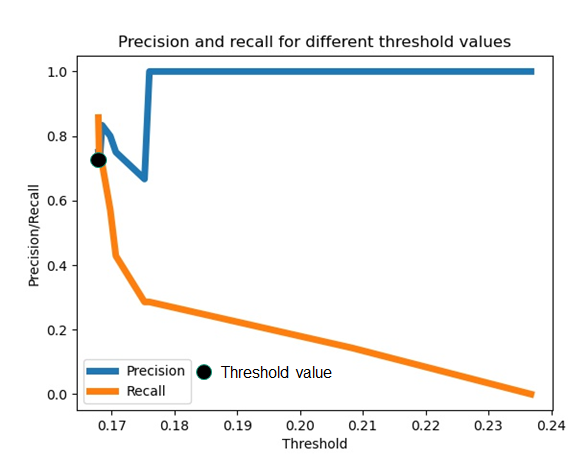
\includegraphics[width=9cm]{stft_threshold_new.png}
    \end{center}
    \caption{Precision and recall curves with respect to threshold of experiment A, the black point marks the threshold value}
    \label{fig:threshold_expa}
\end{figure}



\begin{figure}[t]
\begin{center}
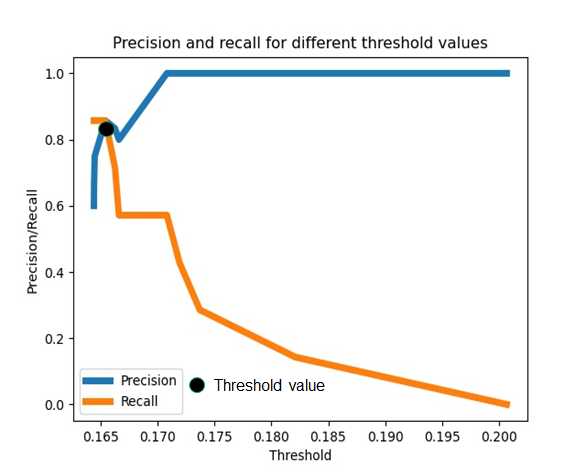
\includegraphics[width=9cm]{order_threshold_new.png}
\end{center}
\caption{Precision and recall curves with respect to threshold of experiment B, the black point marks the threshold value}
\label{fig:threshold_expb}
\end{figure}
 

\begin{figure}[hbt]
\begin{center}
    

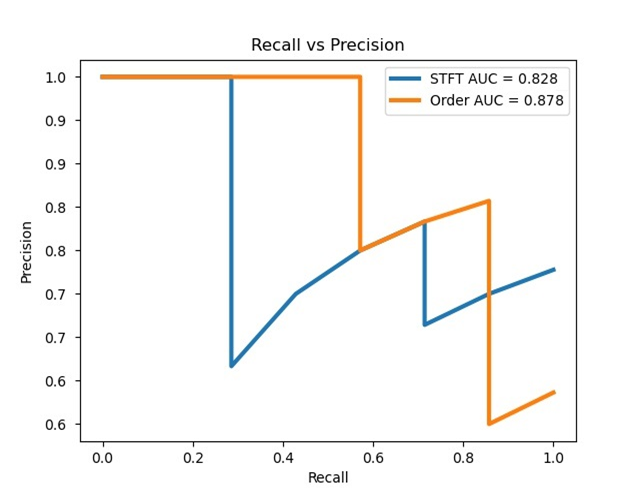
\includegraphics[width=9cm]{auc.png}
\end{center}
\caption{Performance if experiment A and B through AUC precision vs recall curve}
\label{fig:auc_expa_expb}
\end{figure}
    

\begin{figure}[hbt]
\begin{center}
    

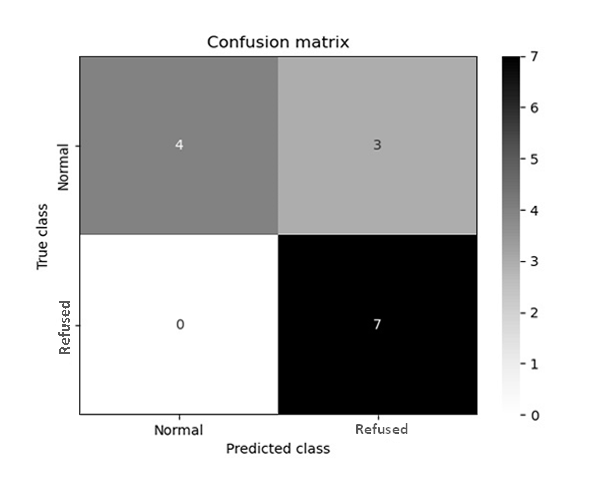
\includegraphics[width=9cm]{conf_matrix_stft.png}
\end{center}
\caption{Confusion matrix experiment A}
\label{fig:conf_matrix_expa}
\end{figure}
Threshold for experiment B is 0.166 as shown in Figure \ref{fig:threshold_expb}. AUC of precision-recall curves are 0.828 (A) and 0.878 (B) as shown in Figure \ref{fig:auc_expa_expb}. Results from experiment B (order features) show a better efficiency in comparison to experiment A. A more detailed analysis of the experiment A can be seen in the confusion matrix of Figure \ref{fig:conf_matrix_expa} where the true class contains annotations identified by an NVH expert through classical analysis and predicted class is the model output. The predicted "refused" label indicates true positives. As shown in Figure. \ref{fig:conf_matrix_expb} all seven refused samples were identified correctly based on the threshold value in Figure \ref{fig:threshold_expa} but three normal samples were also erroneously categorized as refused. In experiment B seven out of six samples were identified correctly while one normal sample was identified as refused and one identified vice versa.    

\begin{figure}[hbt]
\begin{center}
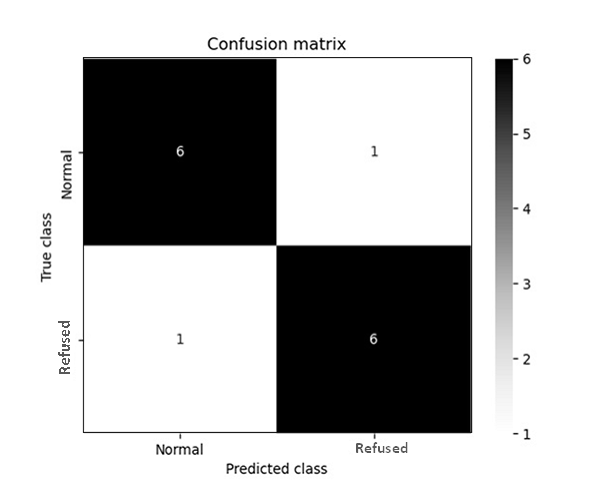
\includegraphics[width=9cm]{conf_matrix_order.png}
\end{center}
\caption{Confusion matrix experiment B}
\label{fig:conf_matrix_expb}
\end{figure}
\FloatBarrier
\section*{Conclusion}
\label{sec:Conclusion}
The best comparative accuracy achieved is 0.878 in experiment B based on order features. A (so called) classical NVH approach requires in depth analyses of simulated, normal and fault-based data using different signal processing techniques and (expensive) expert tools. Unsupervised autoencoders show good results in accuracy compared to classical approaches and "just" require normal data to find noticeable specimen.
Presuming consistency and a certain amount of diversity in the underlying data sets, such data driven methods may help to reduce time consuming data examination tasks for NVH engineers significantly in the (very) near future.    



\section*{Acknowledgment}
\label{sec:Acknowledgment}
This research is conducted in collaboration of Schaeffler AG and Fraunhofer IDMT. Special thanks go to Schaeffler AG for providing datasets and NVH support.  



\begin{thebibliography}{8}
\bibitem{b1}Bengio, Yoshua et al. "Representation learning: A review and new perspectives". IEEE transactions on pattern analysis and machine intelligence 35. 8(2013): 1798–1828.

\bibitem{b2}Rätsch, Gunnar. "A brief introduction into machine learning". Friedrich Miescher Laboratory of the Max Planck Society. (2004).

\bibitem{b3}Koizumi, Yuma et al. "Unsupervised detection of anomalous sound based on deep learning and the neyman–pearson lemma". IEEE/ACM Transactions on Audio, Speech, and Language Processing 27. 1(2018): 212–224.


\bibitem{b4}Knieper, Johannes et al. "Methoden für die akustische Analyse und Bewertung von E-Achs-Getrieben". Deutsche Gesellschaft für Akustik eV: DEGA. (2020).




\bibitem{b5}Shao, Haidong, et al. "A novel deep autoencoder feature learning method for rotating machinery fault diagnosis." Mechanical Systems and Signal Processing 95 (2017): 187-204.




\bibitem{b6}“ASAM MDF.” Association for Standardization of Automation and Measuring Instrument, www.asam.net/standards/detail/mdf/. 

\bibitem{b7}Ribeiro, Alexandrine, et al. "Deep Dense and Convolutional Autoencoders for Unsupervised Anomaly Detection in Machine Condition Sounds." arXiv preprint arXiv:2006.10417 (2020).

\bibitem{b8}Paracha, Abdul Haq Azeem. “Assessment and Application of Machine
Learning Methods to NVH Related Component
Data in the Automotive R\&D Environment.” Technische Universität Ilmenau, 2021. 

\end{thebibliography}

\end{document}
